\section{Cloud Computing}

Im folgenden Unterkapitel werden die Grundlagen und eine Definition des Cloud Computing erarbeitet. Hierbei werden die Grundlegenden Konzepte,
Bereitstellungsmodelle und Abstraktionsebenen des Cloud Computing erläutert.

\subsection{Was ist Cloud Computing}

Nach dem \ac{NIST}, auf dessen Definition sich in jüngerer Literatur häufig bezogen wird \cite[Vgl.][S. 4f]{Reinheimer2018}, ist Cloud Computing ein Modell der Zurverfügungstellung von Computing Ressourcen
(z.B. Netzwerke, Server, Speicher, Anwendungen und Services),die über das Netzwerk erreichbar sind und mit geringem Managementaufwand
schnell freigegeben und bereitgestellt werden können \cite[Vgl.][S. 2]{Mell2011}\cite[Vgl.][S. 5]{Reinheimer2018}.

\begin{wrapfigure}{r}{0.45\textwidth}
\centering
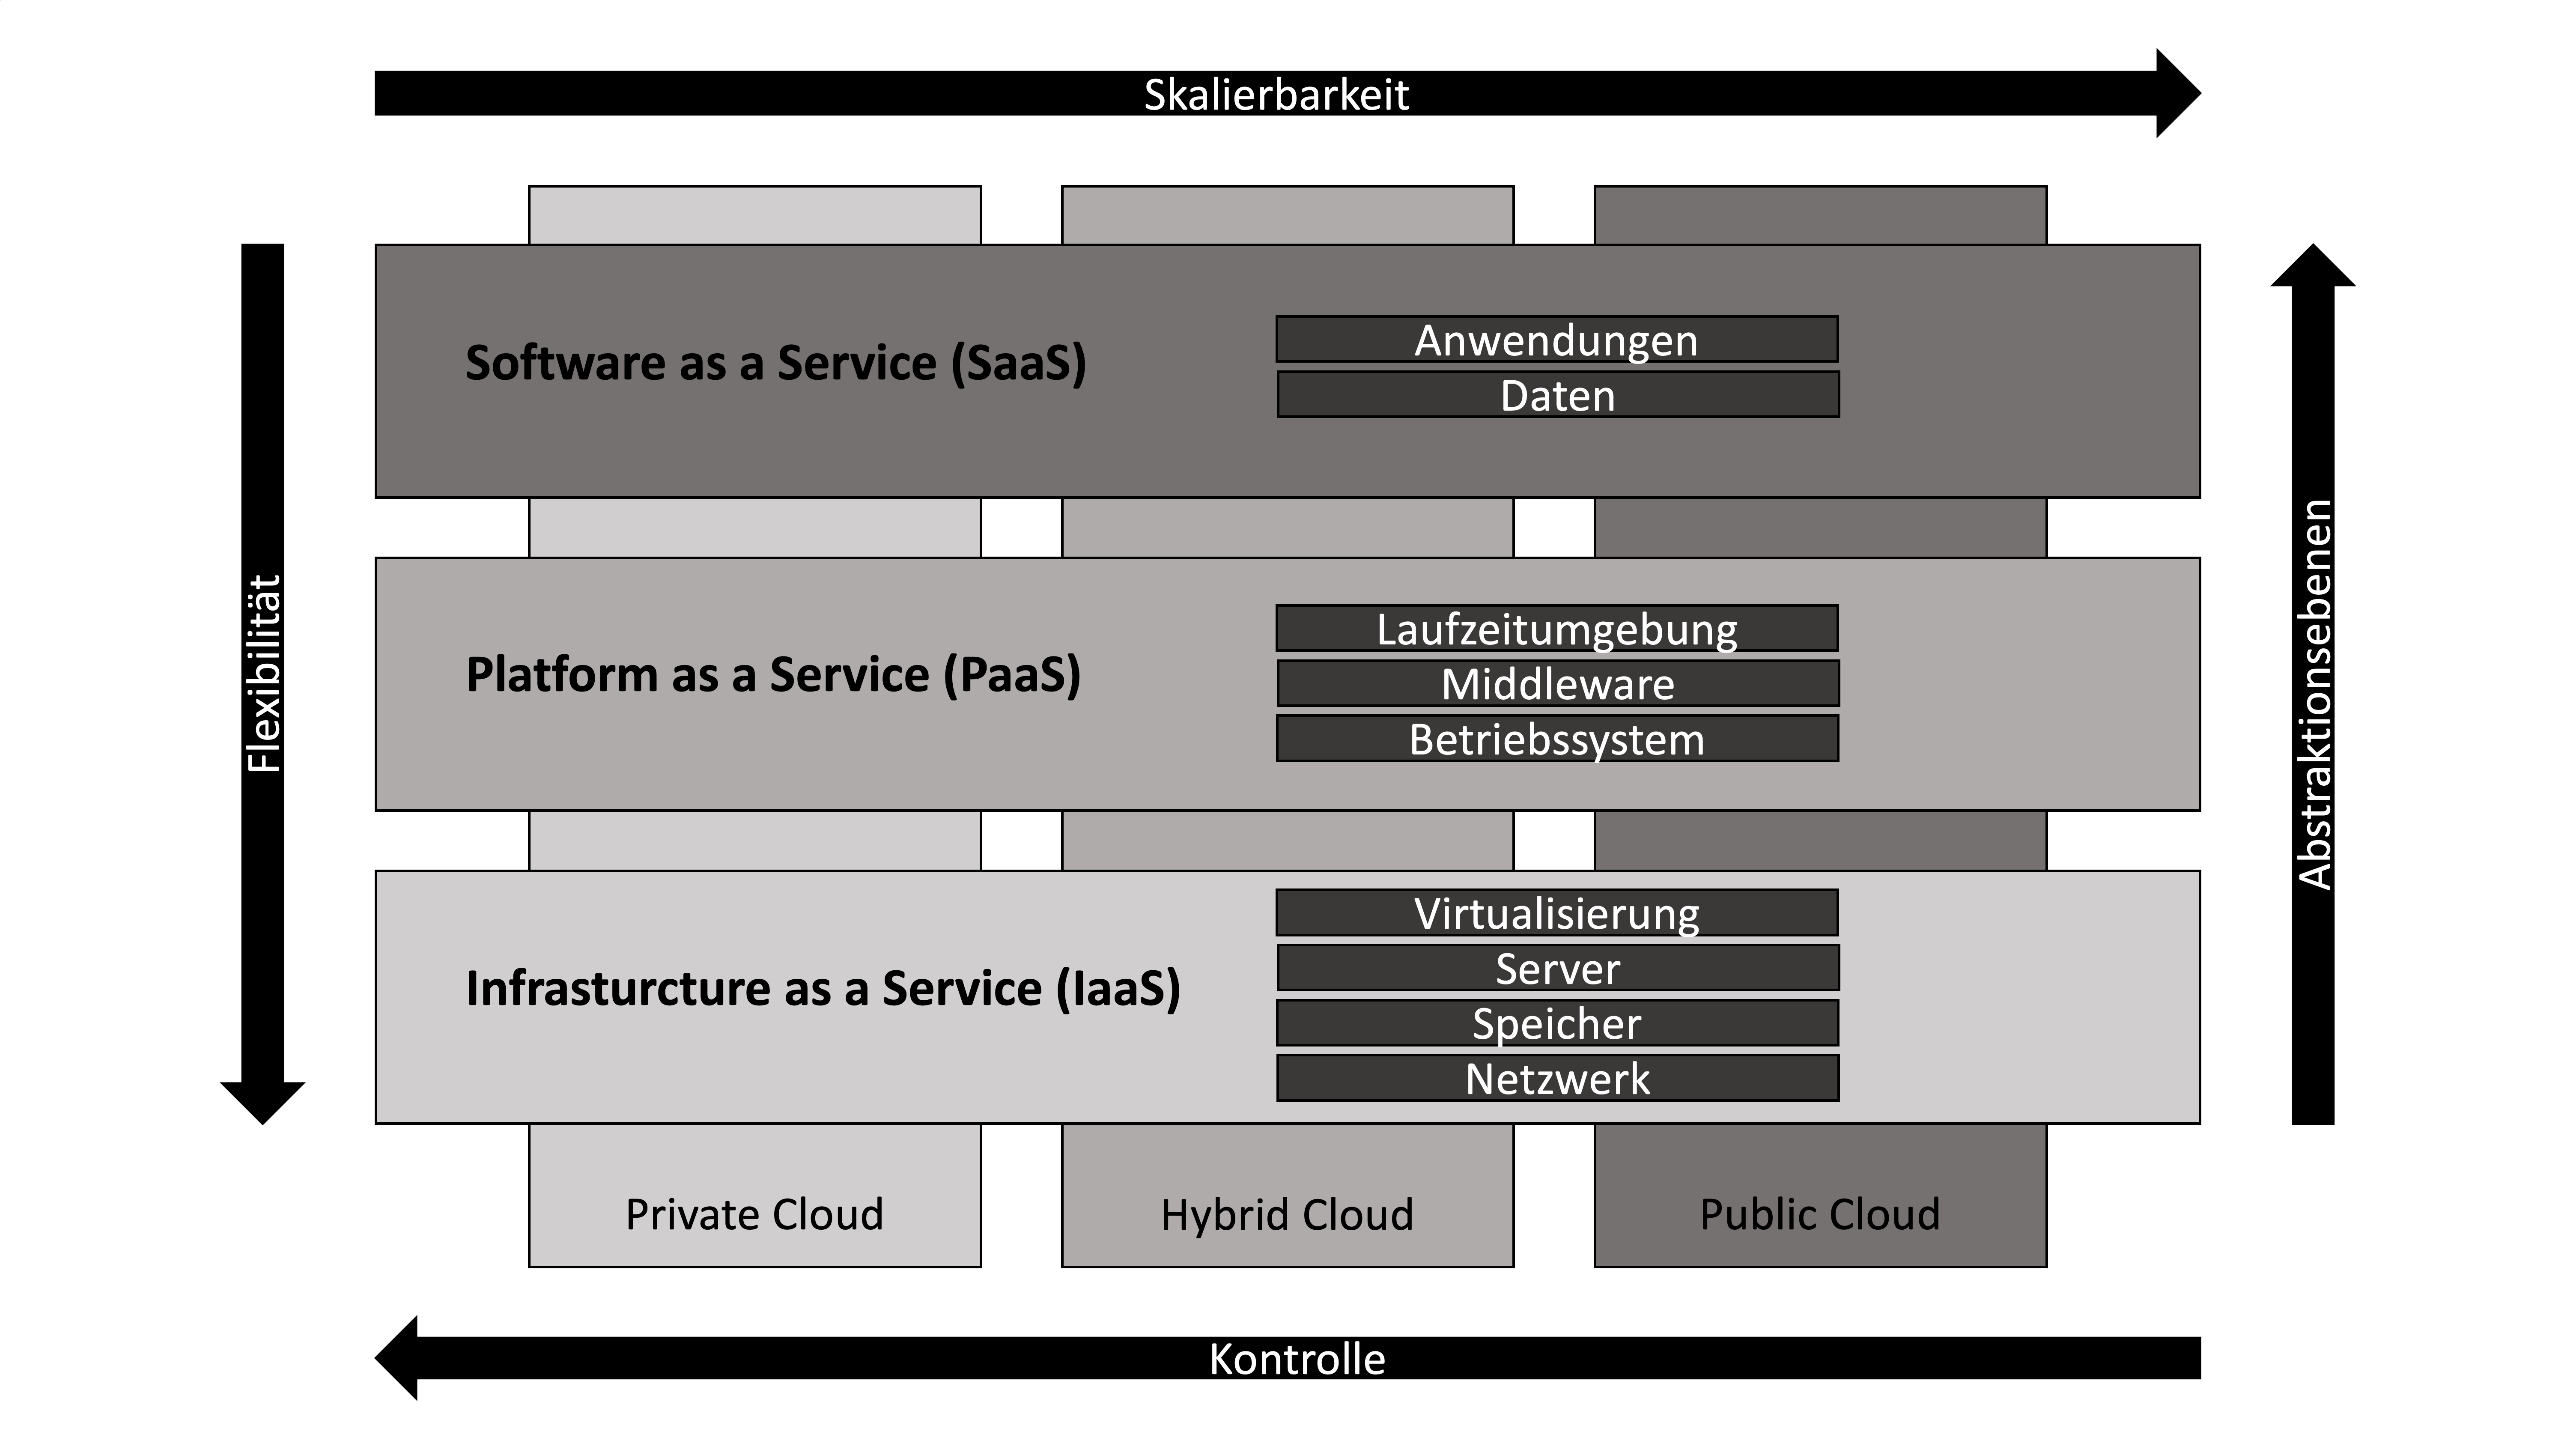
\includegraphics[height=0.3\textwidth]{xaas.png}
\caption{Eine Übersicht der Cloud Service Modelle \cite[Eigene Darstellung nach][S. 33]{Maenhaut2016}\cite[Ergänzt durch][]{Toroman2018}}
\label{fig:XaaS}
\end{wrapfigure}

Nach Hentschel und Leyh (2018), Zhao (2014), Maenhaut (2016) und Surianarayanan (2019) kann man Cloud Services grundsätzlich in drei Abstraktionsebenen einteilen. Diese sind \textbf{\ac{SaaS}},
\textbf{\ac{PaaS}} und \textbf{\ac{IaaS}}, welche auch zu \ac{XaaS} zusammengefasst werden
\cite[Vgl.][S. 9]{Reinheimer2018}\cite[Vgl.][S. 143f]{Zhao2014}\cite[Vgl.][S. 32ff]{Maenhaut2016} und \cite[Vgl.][S. 226ff]{Surianarayanan2019}.

Die in Abbildung \ref{fig:XaaS} dargestellte unterste der drei genannten Abstraktionsschichten ist \ac{IaaS},
welche die Basisinfrastruktur, wie zum Beispiel Netzwerk, Server oder Speicher, bereitstellt.

Diese Infrastruktur kann sowohl physisch als auch virtuell zur Verfügung gestellt werden \cite[Vgl.][S. 9f]{Reinheimer2018}.
Die darüberliegend dargestellte Schicht ist \ac{PaaS}, welche zu der Infrastrukturebene zusätzlich noch eine Basis zur Anwendungsentwicklung bietet, indem zum Beispiel
bereits ein Betriebssystem und Middleware und eine Laufzeitumgebung bereitgestellt werden \cite[Vgl.][S. 10]{Reinheimer2018}.
Die oberste Abstraktionsebene ist \ac{SaaS}, welche standardisierte Anwendungen zur Verfügung stellt und sich somit direkt an den Endnutzer richtet und
ohne Verwaltung der zugrundeliegenden Ressourcen genutzt werden kann. Diese wird vom Provider übernommen.
\cite[Vgl.][S. 11]{Reinheimer2018}.

Generell wird die Cloud darüber hinaus in drei Organisationsdimensionen eingeteilt \cite[Vgl. auch im Folgenden][S. 7ff]{Reinheimer2018}:
\begin{itemize}
\item \textbf{Private Cloud:} Die Private Cloud bietet die exklusive Nutzung durch eine Organisation der darunterliegenden Infrastruktur. 
Die IT-Infrastruktur einer Private Cloud kann entweder im Unternehmenseigenen Rechenzentrum untergebracht oder auch
von Dienstleistern bereitgestellt werden.
\item \textbf{Public Cloud:} In der Public Cloud ist die Infrastruktur für mehr Anwender zugänglich und muss geteilt werden. Dafür muss als Anwender oft
auch nur für die tatsächlich genutzte Leistung gezahlt werden. Da die Infrastutktur jedoch gleichzeitig von vielen genutzt wird, ist zum Beispiel der
Betrieb von sicherheitskritischen Anwendungen schwierig.
\item \textbf{Hybrid Cloud:} Die Hybrid Cloud bildet eine kombinierte Anwendung aus der Public Cloud und der Private Cloud. Diese bietet dem Anwender die
Möglichkeit gewisse Anwendungen in die Public Cloud auszulagern, ohne die Vorteile der Private Cloud für sicherheitsrelevante Anwendungen aufgeben zu msüssen.
Darüber hinaus kann bei einem Hybrid Cloud modell die Rechenleistung der Private Cloud bei Spitzenlast durch die Public Cloud erweitert werden. 
\end{itemize}

\pagebreak

\subsection{Entwicklung des Cloud Computing}

Die Entwicklung des Cloud Computing und dessen Vorgängerkonzepte is bis in die 90er Jahre zurückzuführen.
Ein von Hentschel und Leyh (2018) hervorgehobender Vorgänger ist das sogrnannte Grid Computing.
Damit war bereits eine dezentrale Ressourcenkontrolle mir standardisierten Protokollen und
Schnittstellen realisiert. Das Cloud Computing bietet vergleichbare Eigenschaften, jedoch rückt der
Fokus hier auf wirtschaftliche Kriterien und die Zenralisierung von Ressourcen zum Beispiel in
Rechenzentren \cite[Vgl.][S. 5f]{Reinheimer2018}.

Salesforces ear eines der ersten Unternehmen, welches 1999 Anwendungen über eine Webseite bereitgestellt hat,
gefolgt von den \ac{AWS} in 2002, welche Speicher und Rechenleistung als Services bereitstellten \cite[Vgl.][S. 17f]{Srivastava2018}.

\pagebreak

\subsection{Herausforderungen -> Migration von Legacy Anwendungen}

Aus der vorangehend erläuterten Entwicklung des Cloud Computing ergeben sich verschiedene Herausforderungen.
Darunter fällt unter anderem die Migration von Legacy Anwendungen zu Cloud Anwendungen, welche gegeben durch die verschiedenen Service Level
auf unterschiedlichen Wegen realisiert werden kann.